\begin{figure*}[!t]
\centering
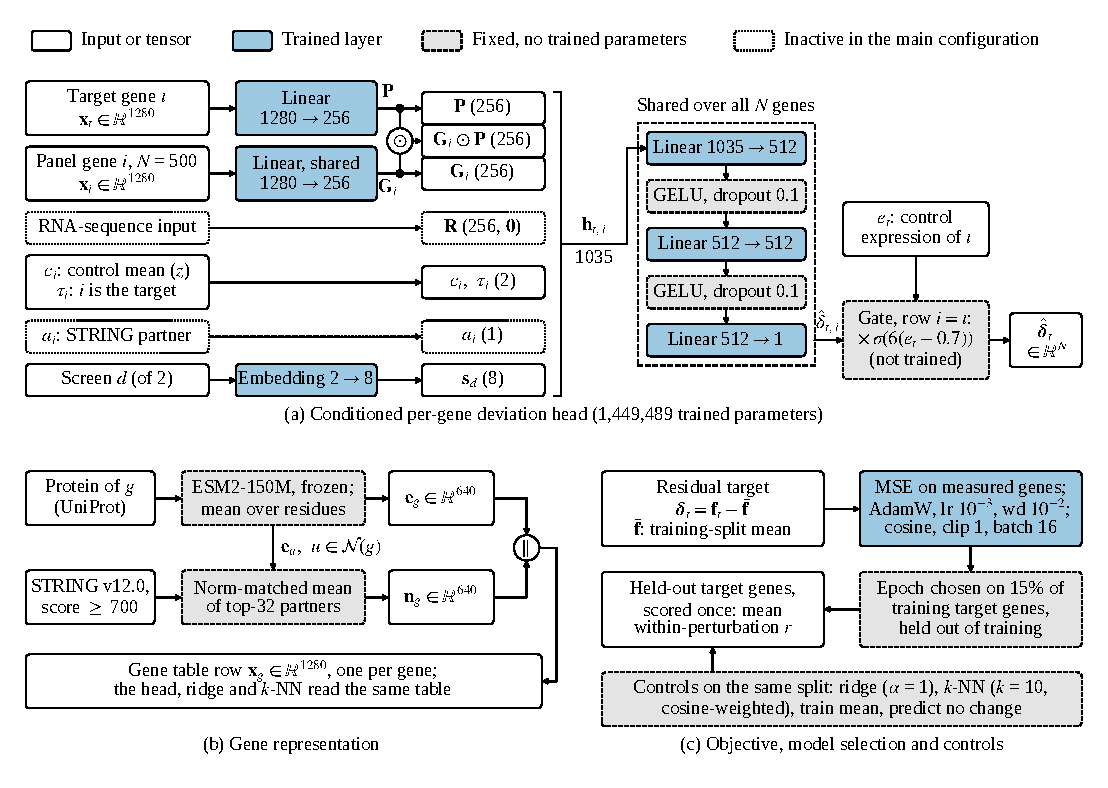
\includegraphics[width=7.16in]{fig_architecture}
\caption{Architecture and training protocol of the conditioned per-gene deviation head. (a) For a perturbation of target gene $t$, the rows of the target ($\mathbf{x}_t$) and of each of the $N=500$ panel genes ($\mathbf{x}_i$) are projected to 256 dimensions by trained linear maps, the panel-gene map shared across genes. Their element-wise product ($\odot$) carries the target--gene interaction. Concatenated with the control expression $c_i$, the target indicator $\tau_i$ and a learned screen embedding $\mathbf{s}_d$, they form the 1035-dimensional feature $\mathbf{h}_{t,i}$, which a 3-layer perceptron with weights shared across genes maps to the residual response $\hat{\delta}_{t,i}$. A fixed sigmoid gate scales the target's own row by its control expression $e_t$. Dotted elements, the RNA-sequence branch and the STRING-partner indicator $a_i$, are inactive in the main configuration and enter as zeros. (b) Each gene's ESM2-150M embedding $\mathbf{e}_g$, the mean over residues, is concatenated ($\Vert$) with the norm-matched mean embedding of its top 32 STRING v12.0 partners (combined score $\geq 700$; zero for genes without partners). The head and the ridge and $k$-NN controls read the same table. (c) The head predicts the residual left after subtracting the mean response of the training split, is trained by mean squared error over measured genes, and its epoch is chosen on an inner validation split of training target genes; held-out target genes are scored once, beside controls evaluated on the identical split. The inner split is held out of training as drawn; the runs reported in Table~I predate that correction and also trained on it (ERRATA E17). The head has 1,449,489 trained parameters with the 1280-dimensional table (1,121,809 with the 640-dimensional ESM2-only table).}
\label{fig:architecture}
\end{figure*}
